% -----------------------------------------------------------------------
% CCN Conference - Extended Abstract Track Template
% For papers up to 2 pages (excluding references); no supplement.
% -----------------------------------------------------------------------
\documentclass{ccn}  % options: submission (default), preprint, extended-abstract
\usepackage{enumitem}

% TODO: For preprints (not accepted), use:
%   \documentclass[preprint]{ccn}

% TODO: For camera-ready extended abstract (after acceptance), use:
%   \documentclass[extended-abstract]{ccn}

% TODO: Add your bibliography file(s).
\addbibresource{ccn_references.bib}

\graphicspath{{figures/}}

% Pink editorial comments
\usepackage{xcolor}
\newcommand{\TS}[1]{\textcolor{magenta}{[TS: #1]}}

\title{Predictive learning explains emergence of objects in infants}

% Authors are automatically anonymized in submission mode.
%
% --- STYLE 1: Single author ---
% \author{Jane Smith \\
%   Department of Neuroscience, University Name \\
%   \email{jane@example.edu}}
%
% --- STYLE 2: Multiple authors, same affiliation (comma-separated, no \And) ---
% \author{Jane Smith, John Doe, and Alice Brown \\
%   Department of Neuroscience, University Name \\
%   \email{\{jane,john,alice\}@example.edu}}
%
% --- STYLE 3: Two authors, different affiliations (use \And) ---
% \author{First Author \\
%   Department of Example, University Name \\
%   \email{first@example.edu}
%   \And Second Author \\
%   Another Department, Another University \\
%   \email{second@example.edu}}
%
% --- STYLE 4: Many authors, traditional format (use \AND for row breaks) ---
% \author{Author One \\
%   Dept of Neuroscience, First Univ \\
%   \email{one@first.edu}
%   \And Author Two \\
%   Dept of Psychology, Second Univ \\
%   \email{two@second.edu}
%   \AND Author Three \\   % \AND starts a new row
%   Dept of Biology, Third Univ \\
%   \email{three@third.edu}
%   \And Author Four \\
%   Dept of Physics, Fourth Univ \\
%   \email{four@fourth.edu}}
%
% --- STYLE 5: Many authors, compact format (recommended for 3+ authors) ---
% Use \affmark{} for superscript numbers, \affiliation{} to define them,
% and optionally \emails{} for a shared email line.
\author{%
  Author One\affmark{1} \And
  Author Two\affmark{1} \And
  Author Three\affmark{2} \And
  Author Four\affmark{2,3} \AND
  Author Five\affmark{3} \And
  Author Six\affmark{4} \And
  Author Seven\affmark{4} \And
  Author Eight\affmark{1,4}%
}
\affiliation{1}{Department of Neuroscience, First University}
\affiliation{2}{Institute for Brain Research, Second University}
\affiliation{3}{Center for Neural Computation, Third University}
\affiliation{4}{Department of Psychology, Fourth University}
\emails{author1@first.edu, author3@second.edu, corresponding@fourth.edu}


\begin{document}

\maketitle

\begin{abstract}
% Organizing visual scenes into objects is fundamental to animal behavior, yet how this capacity develops remains unclear. Human infants initially rely on motion cues to parse objects, whereas sensitivity to static shape cues emerges only later, a trajectory that parallels the earlier maturation of the dorsal stream relative to the ventral stream. Here, we introduce a two-stream neural network in which the ventral and dorsal pathways cooperate to predict future visual input. Trained on videos of moving objects, the model first discovers objects through coherent motion and then develops sensitivity to static shape cues, mirroring human perceptual development. Our results suggest that cross-stream predictive learning, rather than innate perceptual priors, drives the emergence of object representations in early vision.
How do young animals learn to parse visual scenes into objects with so little experience? Human infants initially rely on motion cues to segregate objects, while sensitivity to static shape cues emerges only later --- mirroring the earlier maturation of the dorsal visual stream relative to the ventral stream. Here we introduce a two-stream neural network in which a shape pathway and a motion pathway cooperate to predict future visual input. Trained on videos of moving objects, the model first discovers objects through coherent motion, then develops sensitivity to static shape cues, recapitulating the developmental trajectory observed in infants. These results demonstrate that cross-stream predictive learning is sufficient to produce object representations from a realistic amount of visual experience, without requiring innate perceptual priors.
\end{abstract}

\section{Introduction}

% Organizing a visual scene into structured objects and backgrounds is a crucial step toward intelligent animal behavior. The animal brain is tasked with grouping a complex and ever-changing retinal input into coherent objects despite variations in lighting, occlusion, and perspective. Despite these complexities, even young animals with limited experience with the world achieve this effortlessly. Understanding this mechanism and its development has attracted considerable attention among researchers.
Animals parse visual scenes into objects with remarkably little experience --- human infants can group moving surfaces into coherent objects by four months of age. Yet how this capacity develops from raw sensory input remains an open question.


% One popular theory for this, the Gestalt processing account, posits that perceptual systems of animals have an innate preference for ``simplicity". According to this view, perception is facilitated because objects in the world tend to exhibit simple configurations, such as smooth, continuous contours (``good continuity") and coherent motion among parts (``common fate"). However, studies in developing animals challenge the claim that such grouping principles are innately available. Experiments with infants (\citep{kellman1983perception}) suggest that while they seem to exploit motion-based cues such as common fate, they fail to use static cues such as good continuity. Other forms of synchronous but non-motion changes do not produce the same grouping effects, suggesting a privileged role for motion (\citep{jusczyk1999synchronous}). Therefore, the static grouping cues like good continuity that adults utilize is acquired later through development. Consistent with this interpretation, in adults with congenital blindness who had their vision restored, object parsing was initially only possible when motion cues were present \citep{ostrovsky2009visual}; only with 10-18 months of visual experience did they learn to use static cues like good continuity.
Across species, motion cues precede static shape cues in development. Four-month-old infants group surfaces that move together into a single object but fail to use static alignment cues such as good continuity \citep{kellman1983perception}, and non-motion synchronous changes do not produce the same grouping \citep{jusczyk1999synchronous}. Adults whose congenital blindness was surgically corrected show the same pattern: object parsing initially required motion, and sensitivity to static cues emerged only after months of visual experience \citep{ostrovsky2009visual}. This developmental order mirrors the earlier maturation of the dorsal visual stream relative to the ventral stream \citep{ciesielski2019maturational}, suggesting that motion processing scaffolds the later acquisition of static grouping cues.

% Why and how could motion cues help? Several lines of evidence suggest that the brain continuously predicts the future state of the world (\citep{rao1999predictive, clark2013whatever, caucheteux_evidence_2023}). Such a prediction would inevitably require an understanding of motion. We propose that predictive learning underlies both the acquisition of motion cues and, eventually, the emergence of sensitivity to static cues. Lending credence to this, in infants, when motion is made unpredictable (random video frames instead of smooth continuous motion), visual learning is impaired (\citep{kellman1984perception}). Specifically, we hypothesize that the ventral and dorsal streams cooperate to predict the future visual inputs, and this causes the development of both motion estimation in the dorsal stream, as well as object parsing in the ventral stream.

\begin{figure} %s state preferences regarding figure placement here

% use to correct figure counter if necessary
%\renewcommand{\thefigure}{2}
\begin{center}
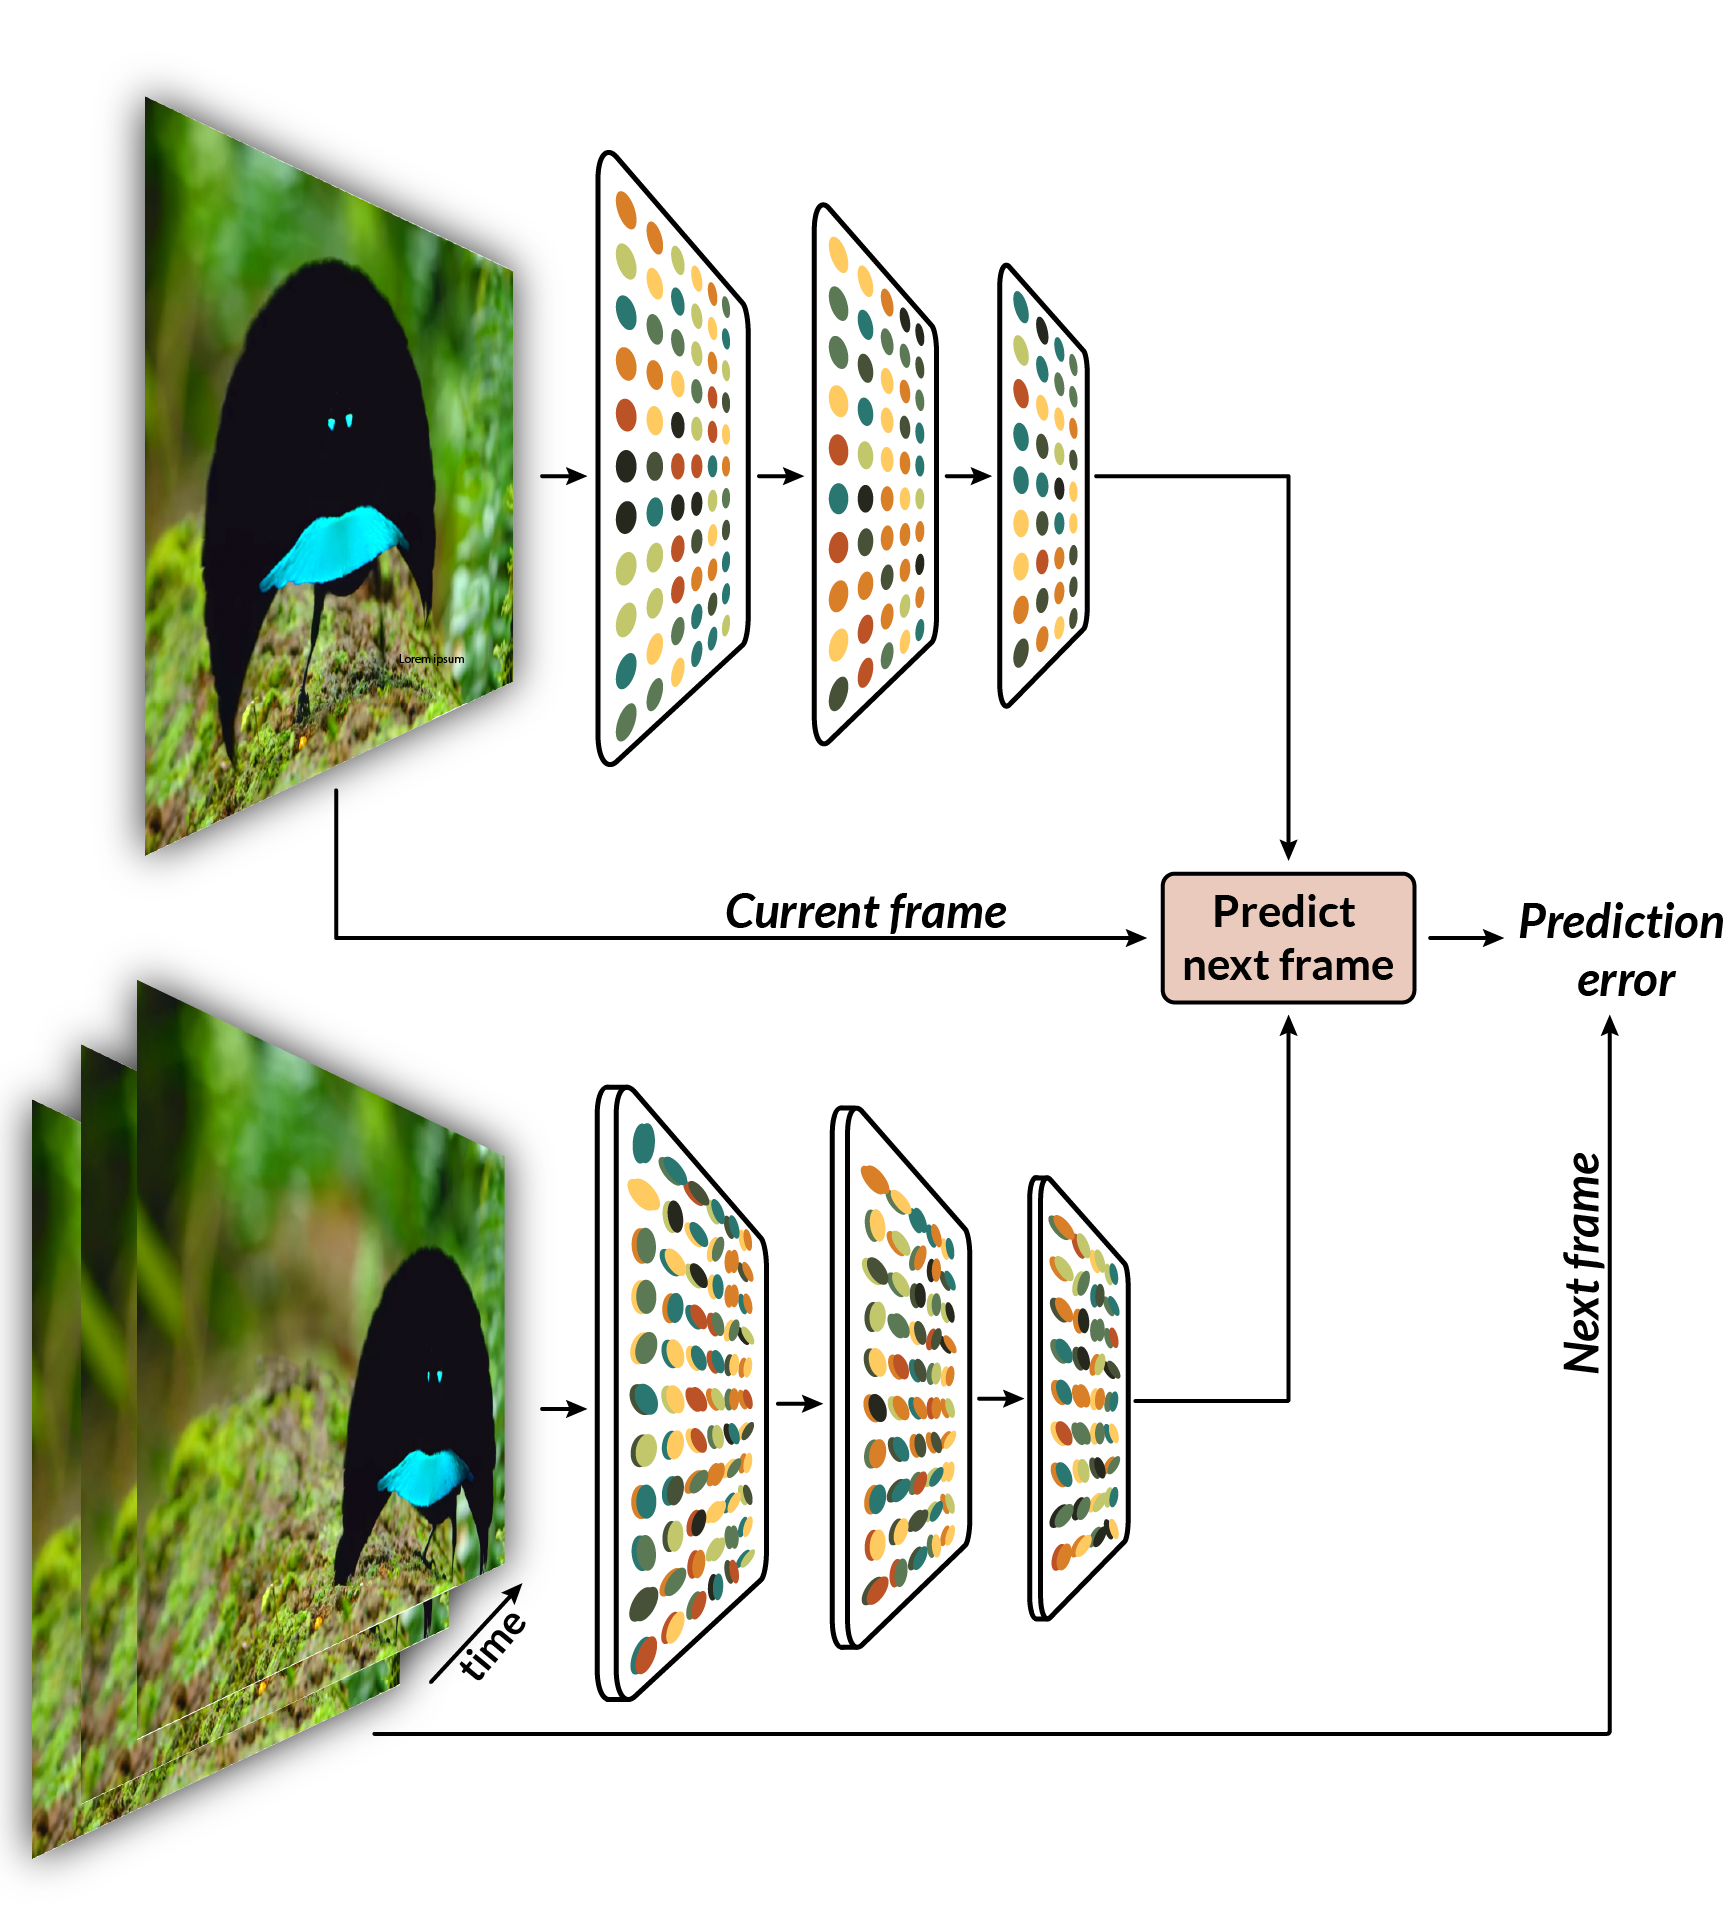
\includegraphics[width=0.30\textwidth]{model.png}
\end{center}

\caption{\textbf{Two stream model of vision.} The model has a separate form and motion pathway which work together to predict the next frame. The prediction error calculated using the predicted and ground truth frames are used to train the model.
}
\label{figmodel} % \label works only AFTER \caption within figure environment
\vspace{-10pt}
\end{figure}

Why should motion be privileged? The brain is thought to continuously predict its future sensory input \citep{rao1999predictive, clark2013whatever, caucheteux_evidence_2023}, and predicting the next visual frame requires estimating what moves and where. We hypothesize that the ventral and dorsal streams cooperate to make this prediction: the dorsal stream estimates motion, while the ventral stream learns to segment the regions that move coherently --- and in doing so, acquires static shape representations as a byproduct. Consistent with this, infant visual learning is impaired when motion is made temporally unpredictable \citep{kellman1984perception}.

% To verify this, we develop a neural network model with two separate visual streams that work together to predict the next frame. When trained to minimize this next-frame prediction error on videos designed to simulate an infant's experience with moving objects, the model recapitulated their behavior -
% \begin{enumerate}
%     \item It discovered the moving objects. That is, it used the common fate cue to group into objects as a consequence of minimizing the prediction error.
%     \item It developed sensitivity to alignment; like human adults, the models eventually became sensitive to the good continuity cue.
% \end{enumerate}
To test this, we build a two-stream neural network whose ventral and dorsal pathways jointly predict the next video frame. Trained on synthetic videos of moving objects, the model first segments objects by coherent motion and later develops sensitivity to static shape cues, recapitulating the developmental trajectory observed in infants.


\begin{figure} %s state preferences regarding figure placement here

% use to correct figure counter if necessary
%\renewcommand{\thefigure}{2}
\begin{center}
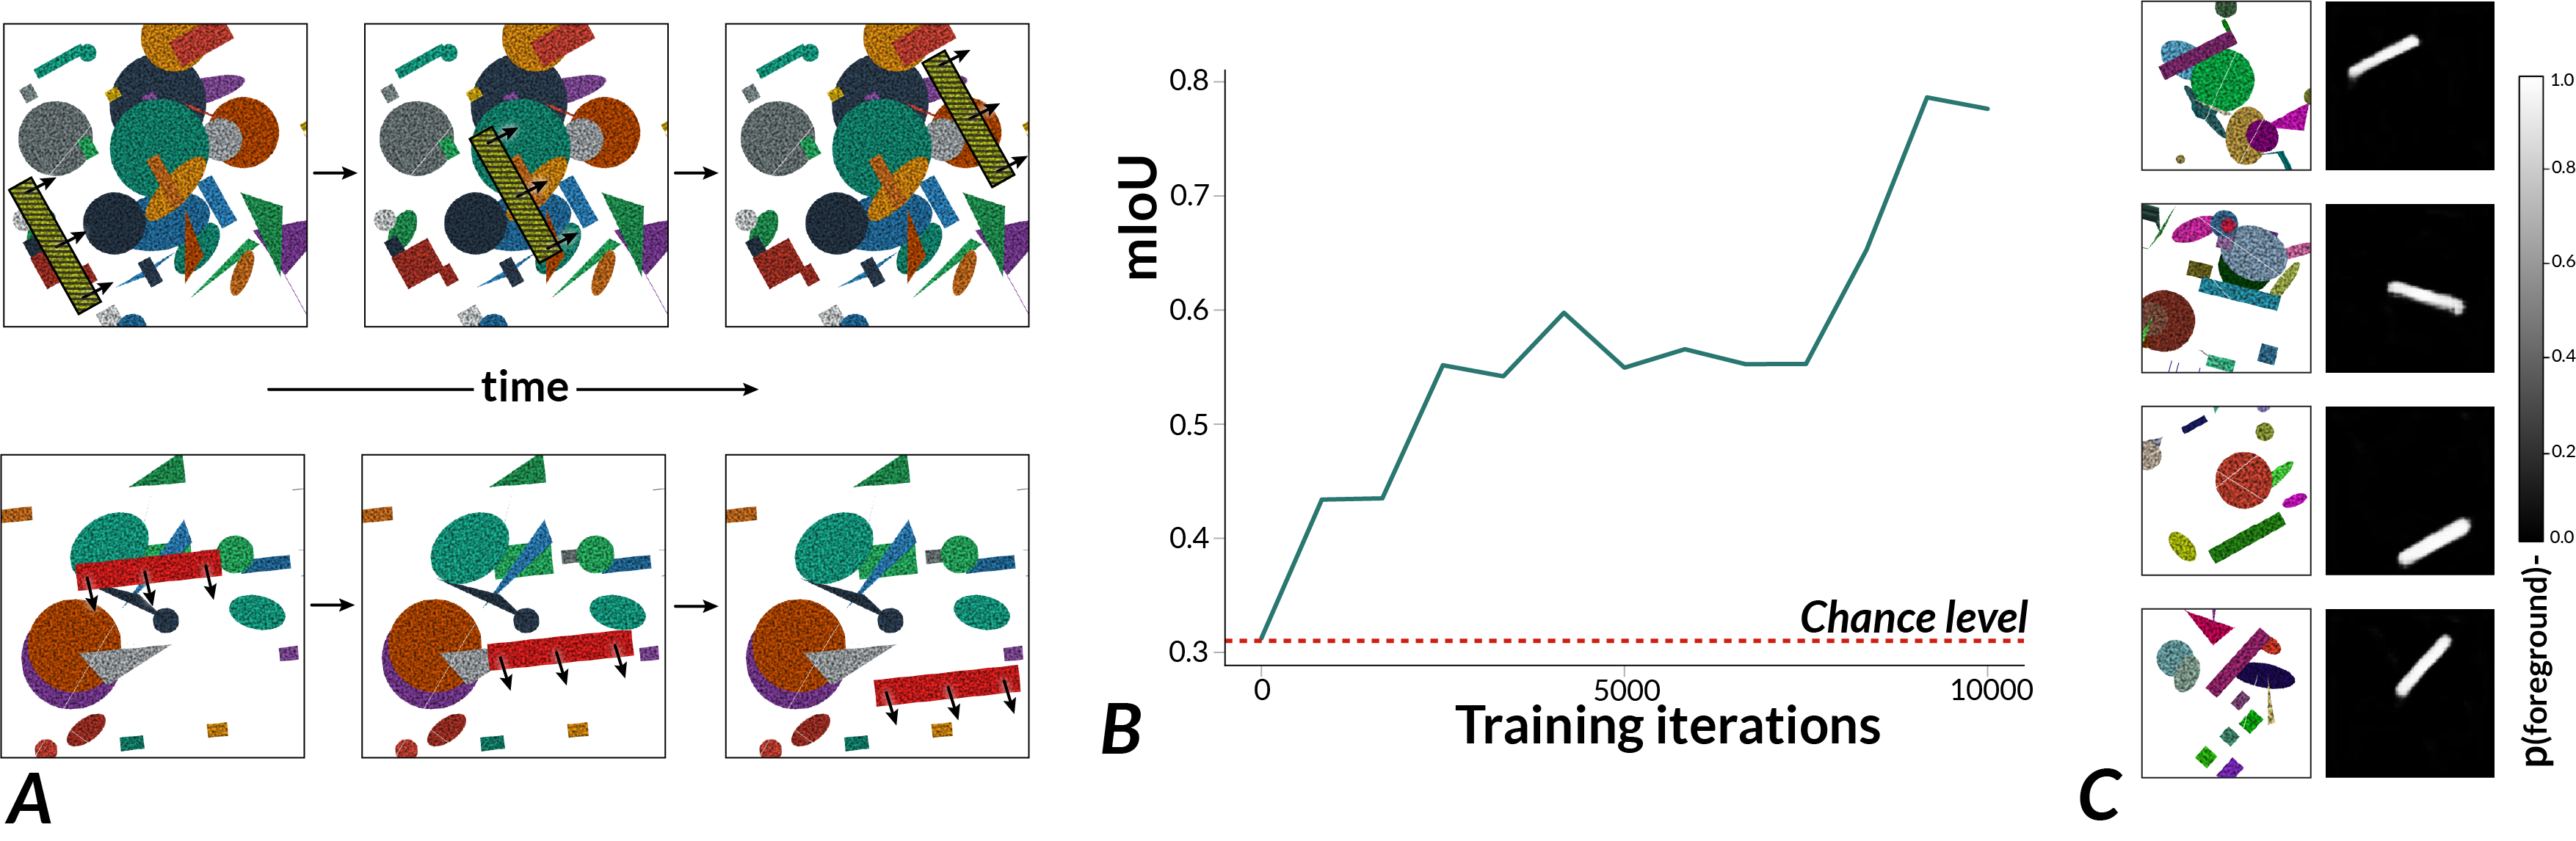
\includegraphics[width=0.5\textwidth]{miou.png}
\end{center}
\caption{\textbf{Predictive learning begets common fate.} \textbf{A.} Example frames of videos used to train the model.
\textbf{B.} Object segmentation accuracy over iterations of prediction error minimization.
\textbf{C.} Example object segmentation predictions.
}

\label{figmiou} % \label works only AFTER \caption within figure environment

\end{figure}
\section*{Results}





\begin{figure*}[h!] %s state preferences regarding figure placement here

% use to correct figure counter if necessary
%\renewcommand{\thefigure}{2}
\begin{center}
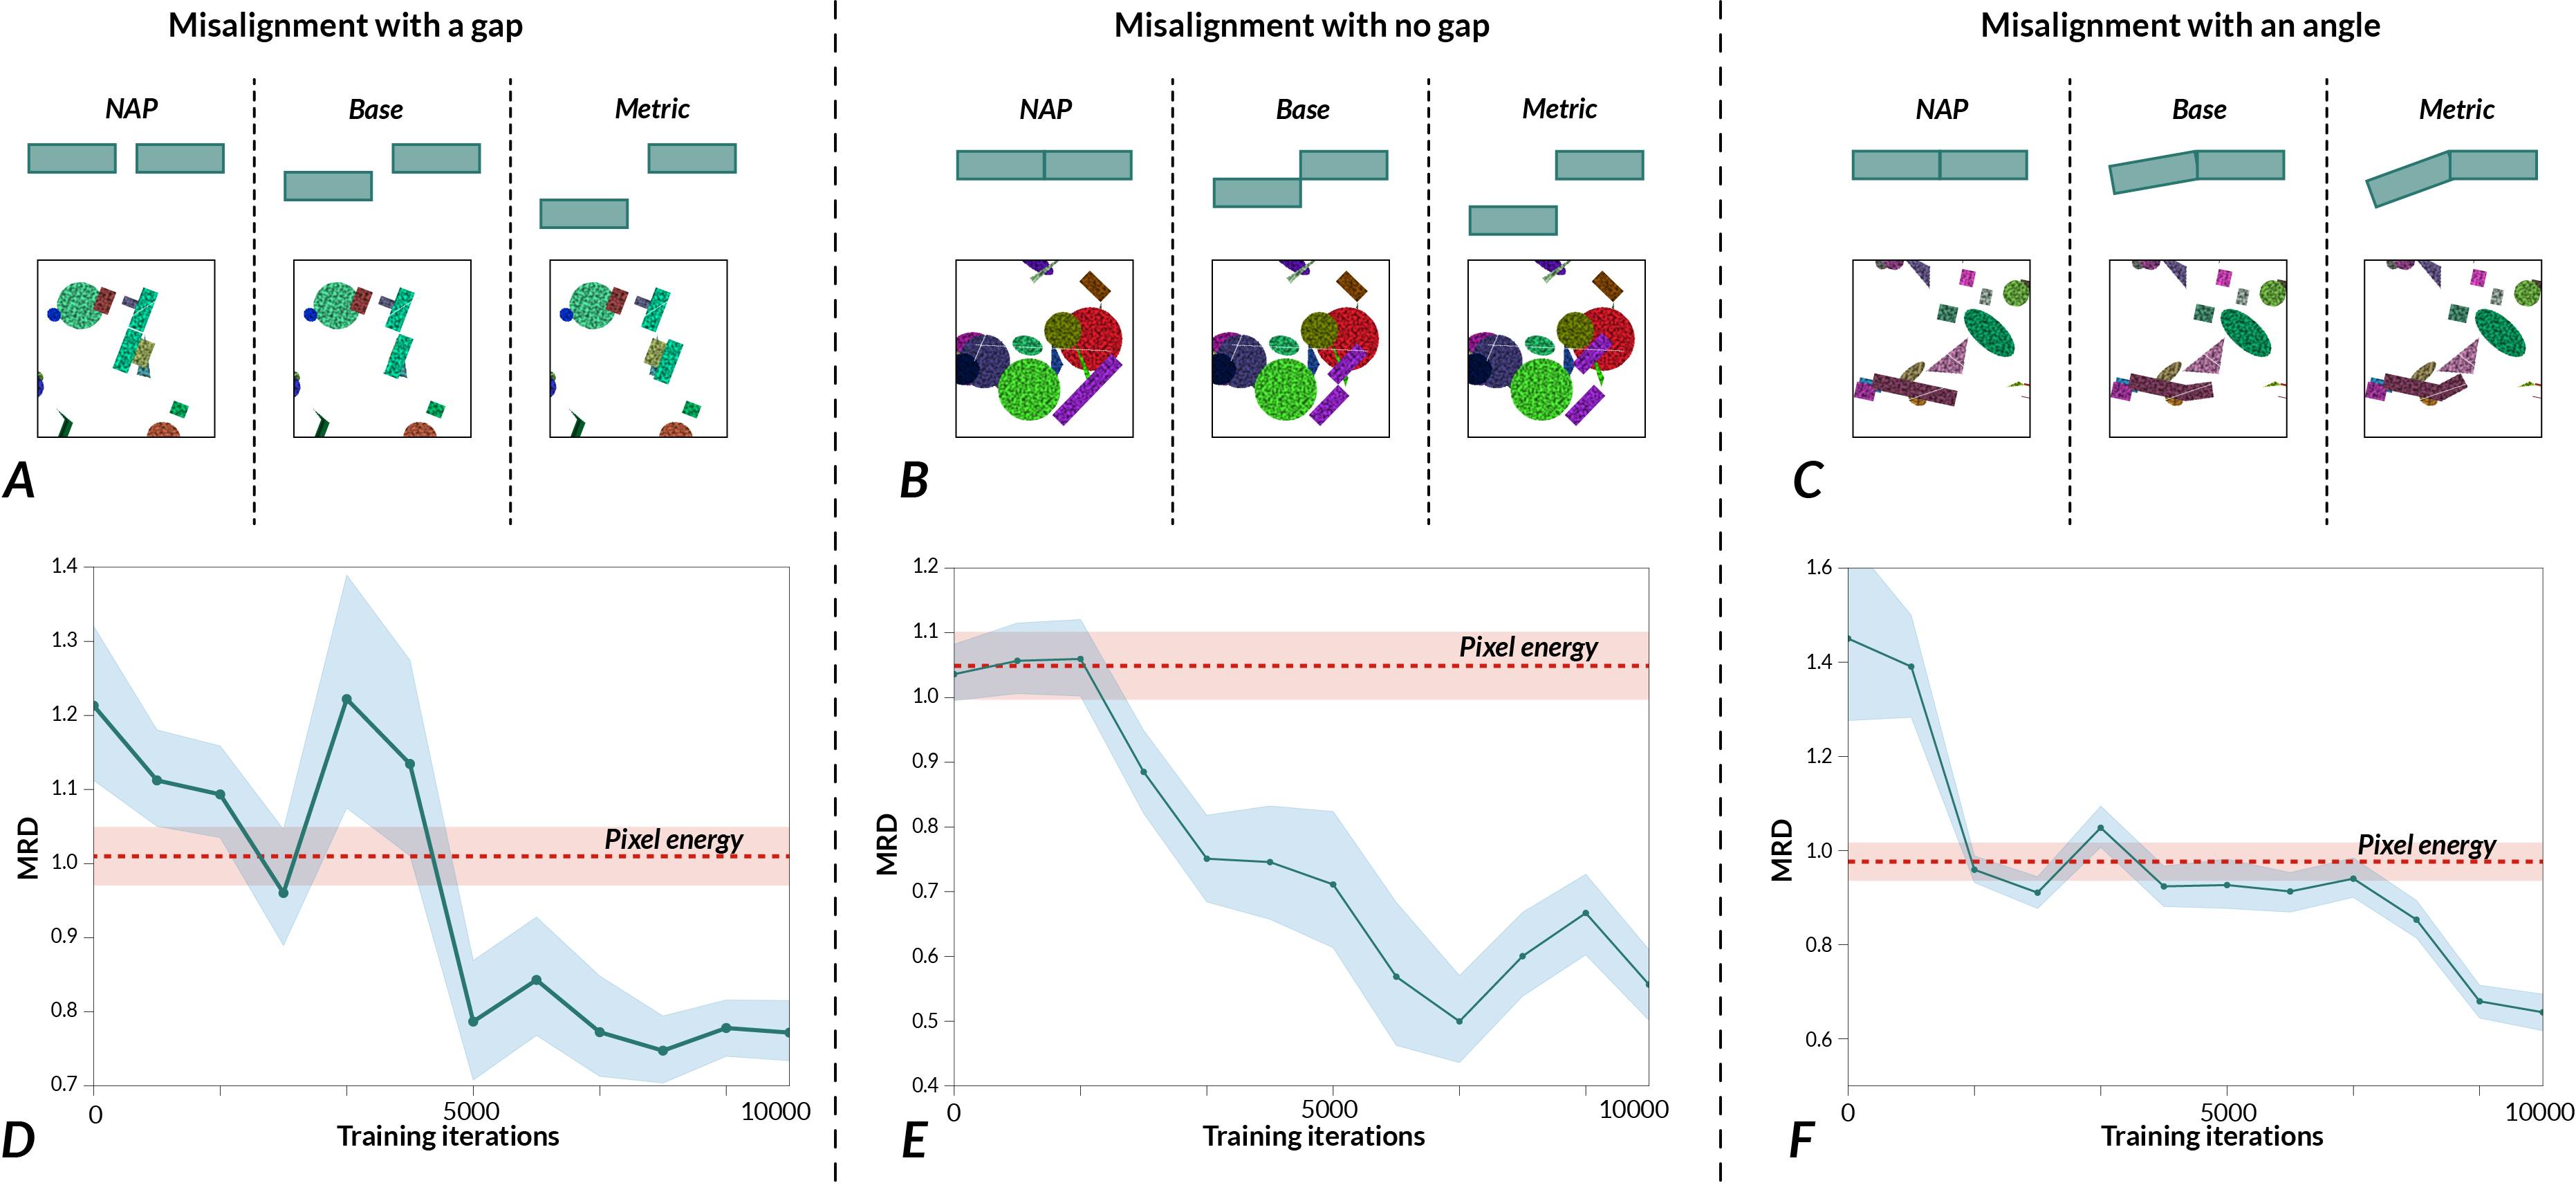
\includegraphics[width=0.8\textwidth]{mrd.png}
\end{center}
\caption{\textbf{Sensitivity to static grouping cues also emerge with prediction error minimization.}
\textbf{A-C.} Example triplets generated to determine sensitivity to static cues in the model. 
\textbf{D-F.} Mean relative dissimilarity (MRD) is defined as the ratio of representational dissimilarities of Base \& Metric pairs to NAP \& Base pairs. }

\label{figmrd} % \label works only AFTER \caption within figure environment

\end{figure*}
\subsection*{A two stream model of vision}

% \TS{Consider adding a small architecture figure (or panel in Fig.~1) showing the two-stream layout.}

% The two-streams hypothesis (\citep{goodale1992separate}) posits that visual information is processed by two distinct pathways, the ventral stream (``what" pathway) and the dorsal stream (``how/where" pathway). The visual stimuli that fall on the retina pass through the LGN and V1 where it splits into the two streams. We model the retina and LGN using a deep neural network ($ \phi_{\theta e}$) that when applied to two temporally consecutive visual stimuli $x_t$ and $x_{t+1}$ produces: $ y_t = \phi_{\theta e}(x_t) \quad y_{t+1} = \phi_{\theta e}(x_{t+1}).$
%
% A subset of the neurons in V1 pass the visual signal into the higher layers of the ventral stream. The subsequent stages (V2, V4, IT) in this stream process the visual information to recognize objects by extracting static cues such as shape, orientation, color, and texture. These cues are utilized to group locations in the visual field into coherent regions, for example, the foreground and the background. We model this using a 3-layer deep convolutional neural network ($ \phi_{\theta v}$) followed by the softmax function which for every spatial location predicts the probability of it being in the foreground rather than the background $f_v = softmax(\phi_{\theta v}(y_t))$
%
% The direction-selective neurons in the V1 innervate into the dorsal stream. MT and MST areas within the dorsal stream are tasked with detecting and processing object motion. Our model of the dorsal stream ($ \phi_{\theta d} $) consisting of a 3-layer 3D convolutional neural network takes in the features of the two consecutive visual stimuli ($y_t$ and $y_{t+1}$) to detect the motion between them $f_d = \phi_{\theta d}(y_t, y_{t+1})$
%
% The static features $f_v$ (estimate of what is expected to move in the frame) and motion features $f_d$ (estimate of what has moved in the two frames) are then combined and used along with the current frame $x_t$ to predict the future frame $h = f_v \circ f_d \quad \hat{x}_{t+1} = predictor(x_t, h) $
%
% This predicted frame can now be compared to the ground truth frame to calculate a prediction error $e$ using a metric $d$. We choose a simple $L^2$ distance as our metric. All the components of our model can be trained using gradient descent to minimize this prediction error ($e = d(\hat{x}_{t+1}, x_{t+1})$).
Motivated by the two-streams hypothesis \citep{goodale1992separate}, our model has three components (Fig.~\ref{figmodel}). An early visual pathway $\phi_{\theta e}$, loosely corresponding to retina through V1, transforms consecutive frames $x_t, x_{t+1}$ into feature maps $y_t, y_{t+1}$ through a hierarchy of simple- and complex-cell-like operations. These features feed into two parallel streams. A shape stream $\phi_{\theta v}$, modeling ventral areas V2/V4/IT, processes a single frame through a hierarchy of feature-selective units and produces a spatial segmentation map via competitive selection: $f_v = \mathrm{softmax}(\phi_{\theta v}(y_t))$. A motion stream $\phi_{\theta d}$, modeling dorsal areas MT/MST, applies direction-selective spatiotemporal filters to the pair $(y_t, y_{t+1})$ to estimate what has moved: $f_d = \phi_{\theta d}(y_t, y_{t+1})$. The shape and motion signals are combined ($h = f_v \circ f_d$) and used alongside the current frame to generate a prediction of the next frame $\hat{x}_{t+1}$. All parameters are learned jointly by minimizing $L^2$ prediction error between $\hat{x}_{t+1}$ and $x_{t+1}$.

%\TS{tried to make this sounds more biological but might not be entirely correct.}







\subsection*{Predictive learning begets common fate.}

% To train the model, we created a new dataset containing objects in motion. We generate 2500 videos (each 20 frames long) where a foreground object (a rectangle) of random color and texture moves over the background consisting of random shapes. The only signal identifying it as a coherent single object was the common motion of its pixels, and the only static cue to identify it was its shape. We train our model to minimize the next frame prediction error on these videos. As the model is training, we compare its estimate of the object ($f_v$) and compare it to the ground truth object segmentation masks (fig).
We train the model on 2500 synthetic videos (20 frames each) in which a textured rectangle moves over a background of random shapes (Fig.~\ref{figmiou}A). The only cue identifying the foreground as a single object is coherent motion; the only static cue is its rectangular shape. With 10,000 iterations of training (minimizing the prediction error), the shape stream's output $f_v$ increasingly aligns with the ground-truth segmentation mask -- a mean Intersection over Union (mIoU) score of around 0.8, well above chance-level (Fig.~\ref{figmiou}B--C), showing that the model discovers objects through motion without any segmentation supervision.


% \TS{Add mIoU numbers here --- what does the model plateau at? How many training iterations / how much data to converge? This grounds the ``realistic amount of experience'' claim from the abstract.} \TS{Control experiment: what happens when frames are temporally shuffled (unpredictable motion)? This would directly parallel Kellman 1984 and close the loop with the intro.}






\subsection*{Predictive learning begets good continuity.}

% To test human subjects' sensitivity to alignment cues, \citep{kim2012greater} created triplets of stimuli - non-accidental property (NAP) condition (edges are aligned), base condition (edges are misaligned by some amount $m$) and metric condition (edges are misaligned by amount $2\times m$). These triplets are created such that in pixel space the difference between NAP stimuli and base stimuli is the same as the difference between base stimuli and metric stimuli. That is, the mean relative dissimilarity (MRD) is close to 1. Despite this, when the subjects are presented these stimuli their lateral occipital cortex (implicated in recognition of object shape) indicated greater sensitivity for NAP to base pair than base to metric pair (\citep{kim2012greater}). If our model developed such sensitivity, MRD calculated using its ventral stream features should be well below 1. To test this, we created similar triplets across three variants (fig).
% \[ MRD_{model} = \frac{1}{N} \sum_{i=1}^{N} \frac{d(\phi_{\theta v}(x_i^{base}), \phi_{\theta v}(x_i^{metric}))}{d(\phi_{\theta v}(x_i^{base}), \phi_{\theta v}(x_i^{NAP})) }\]
Human adults are more sensitive to changes in edge alignment (a non-accidental property, or NAP) than to equivalent pixel-level changes that preserve misalignment \citep{kim2012greater}. To test whether the model develops the same bias, we adopt the triplet paradigm of \citep{kim2012greater}: for each stimulus set, an aligned (NAP) shape, a misaligned (base) shape, and a more-misaligned (metric) shape are constructed so that pixel distances between adjacent pairs are equal (MRD $\approx 1$ in pixel space). If the shape stream is sensitive to alignment, its representational distance for the NAP--base pair should exceed that for the base--metric pair, yielding MRD $ < 1$. We find this across all three stimulus variants (Fig.~\ref{figmrd}D--F), indicating that sensitivity to static grouping cues emerges from predictive learning alone. 

% \TS{Report actual MRD values (mean $\pm$ SE) for each variant --- the reader needs numbers, not just ``we find this.''} \TS{Does this sensitivity emerge later in training than segmentation? If so, say so explicitly --- that's the developmental ordering claim.}

\section{Conclusion}

% Here we introduce a two stream vision model which processes static and moving input separately to predict the future inputs. We show that this model discovers objects because of common motion among their parts and eventually develops sensitivity to static cues much like humans. Together, we use these results to argue that cross-stream predictive learning, rather than innate perceptual priors, drives the emergence of object representations in early vision in developing infants.
A two-stream model trained to predict the next visual frame first discovers objects through coherent motion and then develops sensitivity to static shape cues, recapitulating the developmental trajectory observed in human infants. These results show that the perceptual organization traditionally attributed to innate Gestalt priors can instead emerge from predictive learning over a realistic amount of visual experience. More broadly, they point to cross-stream prediction as a computational principle that may underlie the development of object perception in biological vision. 

% \TS{Ablation: does a single-stream predictive model (no shape/motion split) fail to produce the same developmental ordering? This is the key control for the ``cross-stream'' claim. Even 1--2 sentences of ablation results would strengthen the paper.} 

% \TS{Comparison to baselines: how do PredNet or other single-stream predictive models perform on these tasks? Naming specific models that fail (as in the full paper with DINOv2, SAM, etc.) would sharpen the contribution.} \TS{Brief limitation/future direction: e.g., extending to more complex natural scenes, or testing whether the model also explains chick imprinting behavior (teasing the full paper).}





\printbibliography

\end{document}
